\documentclass[10pt]{article}
\usepackage[margin=0.62in]{geometry}
\usepackage{booktabs,enumitem,fancyhdr,graphicx,tabularx,titlesec}
\usepackage[hidelinks]{hyperref}
\graphicspath{{docs/lessons/assets/}{../assets/}}
\hypersetup{pdftitle={ADK Lesson 053: Known Local Infrared Emission},
 pdfauthor={Kevin Shanahan},
 pdfsubject={Closed symbolic catalog, transactional envelope intent, cancellation, and inert deterministic replay},
 pdflang={en-US}}
\pagestyle{fancy}\fancyhf{}
\lhead{\textsc{ADK Lesson 053}}\rhead{Known Local IR Emission}
\cfoot{\thepage}\setlength{\headheight}{14pt}
\setlength{\parindent}{0pt}\setlength{\parskip}{3pt}
\setlist{nosep,leftmargin=1.45em}
\titleformat{\section}{\Large\bfseries}{\thesection}{0.5em}{}
\newcommand{\lessonbox}[1]{\begin{center}\fbox{\parbox{0.92\linewidth}{#1}}\end{center}}
\newcommand{\blankline}{\rule{0.78in}{0.4pt}}

\begin{document}
\small
\begin{center}
 {\Huge\bfseries Known Local Infrared Emission}\\[3pt]
 {\Large Schedule one closed-catalog envelope without emitting light}\\[7pt]
 \fbox{\textbf{E0 SYMBOLIC INTENT --- NO EMITTER, CARRIER, PIN, OR TIMER}}
\end{center}
\begin{tabularx}{\linewidth}{@{}>{\bfseries}l X >{\bfseries}l X@{}}
Lesson & 053 --- component & Time & 110--150 minutes\\
Prerequisite & explicit modular time & Board & compile-only Mega replay\\
Evidence & named memory result cells & Boundary & immutable local catalog\\
\end{tabularx}

\lessonbox{\textbf{Responsibility.} \texttt{KnownIrEmissionPolicy} turns one
firmware-authored symbolic command into bounded
\texttt{CarrierOn}, \texttt{CarrierOff}, or \texttt{Inactive} memory intent.
It owns no output, timer, pin, interrupt, carrier, emitter, receiver, supply,
or optical path.}

\section{Select only from the closed catalog}
The four harmless local symbols are \texttt{StationPing},
\texttt{StationReady}, \texttt{StationCancel}, and
\texttt{StationAcknowledge}. The catalog revision and digest cover every
semantic entry field. Runtime code cannot add, edit, import, learn, or infer
an entry.

\begin{center}
% ADK visual: pencil
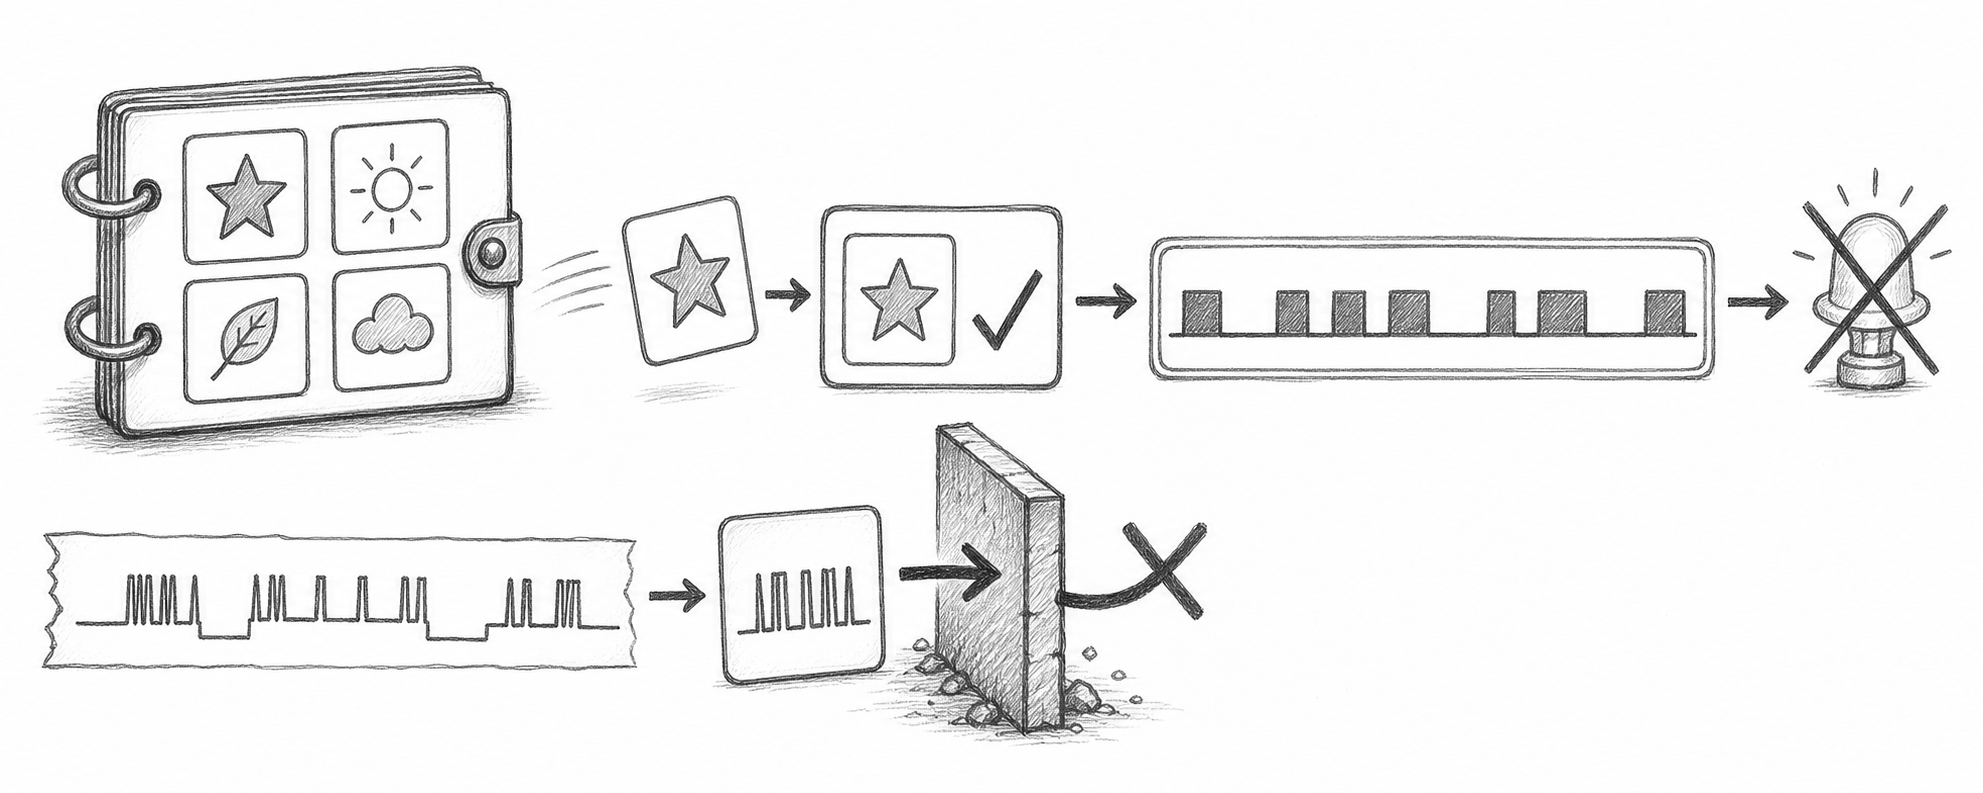
\includegraphics[width=0.98\linewidth,height=0.30\textheight,
 keepaspectratio]{053-closed-catalog-pencil.png}

\small\textit{Alternative text: a closed graphite catalog selects one symbol
card, retains and checks its preview, and derives a bounded mark-space
envelope ending inactive. A raw pulse strip below meets a solid barrier and
cannot enter the catalog path.}
\end{center}

No public request accepts a pulse frame, captured view, raw address or command,
duration array, waveform, or arbitrary bytes. Lesson 052 evidence therefore
has no type-directed path to transmission.

\section{Prepare, verify, then commit once}
\texttt{prepare(codeId, transactionId, now)} reserves one candidate bound to
the policy instance, configuration revision, epoch, policy and candidate
generations, transaction ID, selected symbol, catalog identity, start and
completion times, and candidate digest.

\begin{enumerate}
 \item Prepare exactly one symbolic request; a second request reports busy.
 \item Inspect the retained preview without mutating active policy.
 \item Require \texttt{canCommit()} at the exact proposed start time.
 \item Commit the unchanged preview once, or cancel it before commit.
 \item Derive the envelope intent true at each supplied time directly.
\end{enumerate}

Foreign, reconstructed, changed, stale, consumed, cancelled, or earlier-epoch
previews reject without mutation. A delayed commit is not backdated or shifted;
prepare a fresh candidate for a later start.

\section{Never catch up missed transitions}
The policy does not replay carrier cycles. It computes the current envelope
phase in constant work. A late update publishes only the intent true at that
time. At or after completion it remains \texttt{Inactive}; no missed burst is
compressed into the next call.

\begin{tabularx}{\linewidth}{@{}l X X@{}}
\toprule
Boundary & Prediction & Interpretation\\
\midrule
exact start & first envelope intent & not electrical carrier start\\
mark/space edge & one current intent & no loop over prior edges\\
repeated time & byte-identical state & no duplicate transition\\
late service & current phase or complete & no catch-up burst\\
exact completion & inactive, complete & not proof of optical darkness\\
half-range ambiguity & reject atomically & never guess ordering\\
\bottomrule
\end{tabularx}

\section{Make cancellation dominant}
Before commit, exact candidate cancellation records
\texttt{CancelledBeforeCommit} and never publishes \texttt{CarrierOn}. After
commit, cancellation by the exact transaction publishes \texttt{Inactive}
immediately and records \texttt{CancelledActive}. A matching repeated terminal
cancellation is idempotent.

At a shared timestamp, a composing coordinator consumes cancellation before
commit, update, or application of intent. Direct callers that split those
inputs cannot claim call-order-independent dominance. Shutdown also publishes
inactive intent and advances generation so old previews cannot revive.

\newpage
\section{Run the secret-handshake workbook}
\begin{enumerate}
 \item Initialize. Predict idle lifecycle, inactive intent, immutable catalog
       revision, and catalog digest.
 \item Prepare \texttt{StationPing}. Try a second prepare, foreign preview,
       changed preview, stale generation, and a delayed commit.
 \item Commit at the exact start. Sample every representative mark and space
       boundary without iterating missed intervals.
 \item Cancel a prepared request, then cancel an active request. Collide
       cancellation with a due transition and give cancellation precedence.
 \item Update after completion and verify that no catch-up burst appears.
 \item Exercise timestamp rollover, regression, and half-range ambiguity.
 \item Shutdown and reinitialize. Verify that the prior preview stays stale.
\end{enumerate}

\begin{tabularx}{\linewidth}{@{}X X X X X@{}}
\toprule
time & symbol & phase & envelope intent & transaction\\
\midrule
\rule{0pt}{16pt}\blankline & \blankline & \blankline & \blankline & \blankline\\[8pt]
\blankline & \blankline & \blankline & \blankline & \blankline\\[8pt]
\blankline & \blankline & \blankline & \blankline & \blankline\\
\bottomrule
\end{tabularx}

\section{Separate acquisition evidence from safe-state evidence}
\textbf{Acquisition prediction.} A supported configuration, nonzero epoch,
and immutable catalog identity allow the pure policy to initialize.

\textbf{Acquisition observation.} Host tests inspect lifecycle, catalog
identity, preview bindings, transaction attribution, phase, deadline, and
envelope intent in memory.

\textbf{Acquisition interpretation.} Success proves closed-catalog
transaction and timing semantics only. It does not acquire a timer, pin,
emitter, driver, receiver, supply, or carrier endpoint.

\textbf{Safe-state prediction and observation.} Construction, failed
initialization, cancellation, completion, fault, shutdown, and restart publish
\texttt{Inactive} memory intent. That is not an emergency stop, power removal,
or electrical proof that an emitter is dark.

\section{Read the conservative resource evidence}
A fresh final canonical Mega 2560 build measures 4,854 bytes of flash and
276 bytes of static SRAM with Arduino AVR core 1.8.8 and avr-gcc 7.3.0.
\texttt{sizeof(KnownIrEmissionPolicy)} is 74 bytes. Conservative compiler
stack evidence estimates about 155 bytes on the measured deepest analyzed
path.

These values are compiler evidence for the exact enhanced example, source,
toolchain, optimization, and fixture. They are not runtime high-water
measurements, proof of every interrupt schedule, or evidence of a carrier or
emitter. Re-measure after any source, core, compiler, flag, or composition
change.

\section{Keep E1 explicitly open}
No exact emitter is selected, and the authorized kit inventory does not
establish one. E1 must qualify the exact emitter, driver, resistor, supply,
carrier timer/channel/pin, receiver, observation path, optical geometry,
default-off behavior, and bench acceptance. Current limiting and bounded duty
reduce exposure; they do not establish eye safety. This lesson makes no
eye-safety claim and supplies no wiring or formal schematic.

\section{Record the E0 result}
\begin{itemize}
 \item acquisition status: \blankline\quad catalog revision: \blankline
 \item prepared symbol: \blankline\quad transaction: \blankline
 \item completion intent: \blankline\quad cancellation result: \blankline
 \item safe-state result: \blankline
\end{itemize}

Lesson 054 may map one fixed valid receive symbol to a different fixed local
symbol. Repeat, unknown, malformed, self-echo, and arbitrary captured data
remain ineligible.

\end{document}
